% Standalone vector figure extracted from manuscript.tex.
% Rebuild all figures from the project root: bash tkz/build.sh
\documentclass[tikz,border=2pt,class=IEEEtran]{standalone}
\usepackage{amsmath,amssymb,amsfonts}
\usepackage{xcolor}
\usetikzlibrary{positioning,arrows.meta,calc,backgrounds}

% Match the manuscript's IEEE Access text and math font settings.
\renewcommand{\textbf}[1]{{\fontseries{b}\selectfont #1}}
\renewcommand{\textit}[1]{{\itshape #1}}
\makeatletter
\AtBeginDocument{%
  \fontencoding{T1}\rmfamily\fontseries{m}\fontsize{10}{12}\selectfont
  \gdef\operator@encoding{T1}%
  \gdef\encodingdefault{T1}}
\makeatother

% ---- shared palette for review figures ----
\definecolor{cVLA}{HTML}{34618E}   % VLA lane / policy blue
\definecolor{cWM}{HTML}{9E4A3F}    % world-model lane
\definecolor{cCONV}{HTML}{5E4B8B}  % convergence purple
\definecolor{cGood}{HTML}{3A7D44}  % verified green
\definecolor{cWarn}{HTML}{B07A2A}  % caution amber
\definecolor{cPale}{HTML}{F2F0EA}  % pale panel fill
\tikzset{
  fnode/.style={draw=black!55, fill=white, rounded corners=1.5pt,
                inner sep=2.5pt, align=center, font=\fontsize{8}{9.5}\selectfont},
  flane/.style={draw=none, rounded corners=2pt, inner sep=3pt,
                align=center, font=\fontsize{8}{9.5}\selectfont\bfseries, text=white},
  farr/.style={-{Stealth[length=2mm]}, thick, black!60},
}


\newcommand{\figfont}{\fontsize{8}{9.5}\selectfont}

\begin{document}

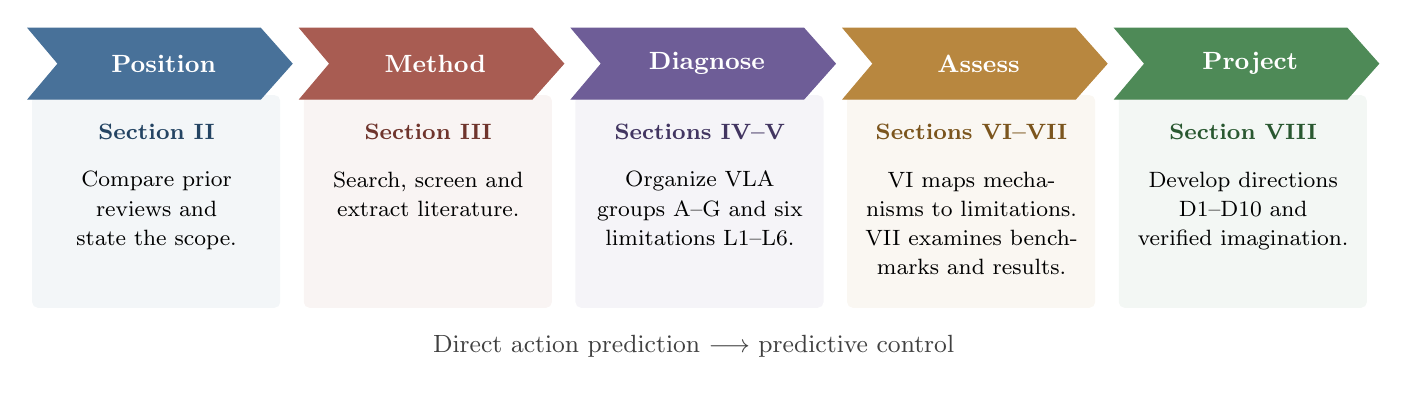
\begin{tikzpicture}[font=\fontsize{8.5}{10.5}\selectfont]
\foreach \x/\col/\head/\sec/\body in {
 0/cVLA/Position/{Section II}/{Compare prior reviews and state the scope.},
 3.45/cWM/Method/{Section III}/{Search, screen and extract literature.},
 6.9/cCONV/Diagnose/{Sections IV--V}/{Organize VLA groups A--G and six limitations L1--L6.},
 10.35/cWarn/Assess/{Sections VI--VII}/{VI maps mechanisms to limitations. VII examines benchmarks and results.},
 13.8/cGood/Project/{Section VIII}/{Develop directions D1--D10 and verified imagination.}}{
 \begin{scope}[xshift=\x cm]
 \fill[\col!6,rounded corners=2pt] (.05,-2.65) rectangle (3.2,.05);
 \path[fill=\col!90,draw=\col!90] (0,0)--(2.95,0)--(3.35,.45)--(2.95,.9)--(0,.9)--(.38,.45)--cycle;
 \node[text=white,font=\fontsize{9}{11}\selectfont\bfseries] at (1.72,.45) {\head};
 \node[font=\fontsize{8.5}{10.5}\selectfont\bfseries,align=center,text=\col!70!black] at (1.63,-.42) {\sec};
 \node[text width=27mm,align=center,anchor=north] at (1.63,-.8) {\body};
 \end{scope}}
\node[font=\fontsize{9}{11}\selectfont,text=black!75] at (8.45,-3.14)
 {Direct action prediction $\longrightarrow$ predictive control};
\end{tikzpicture}
\end{document}
